\section{Inverted Double Pendulum model} 
\begin{figure}[H]
	\centering
	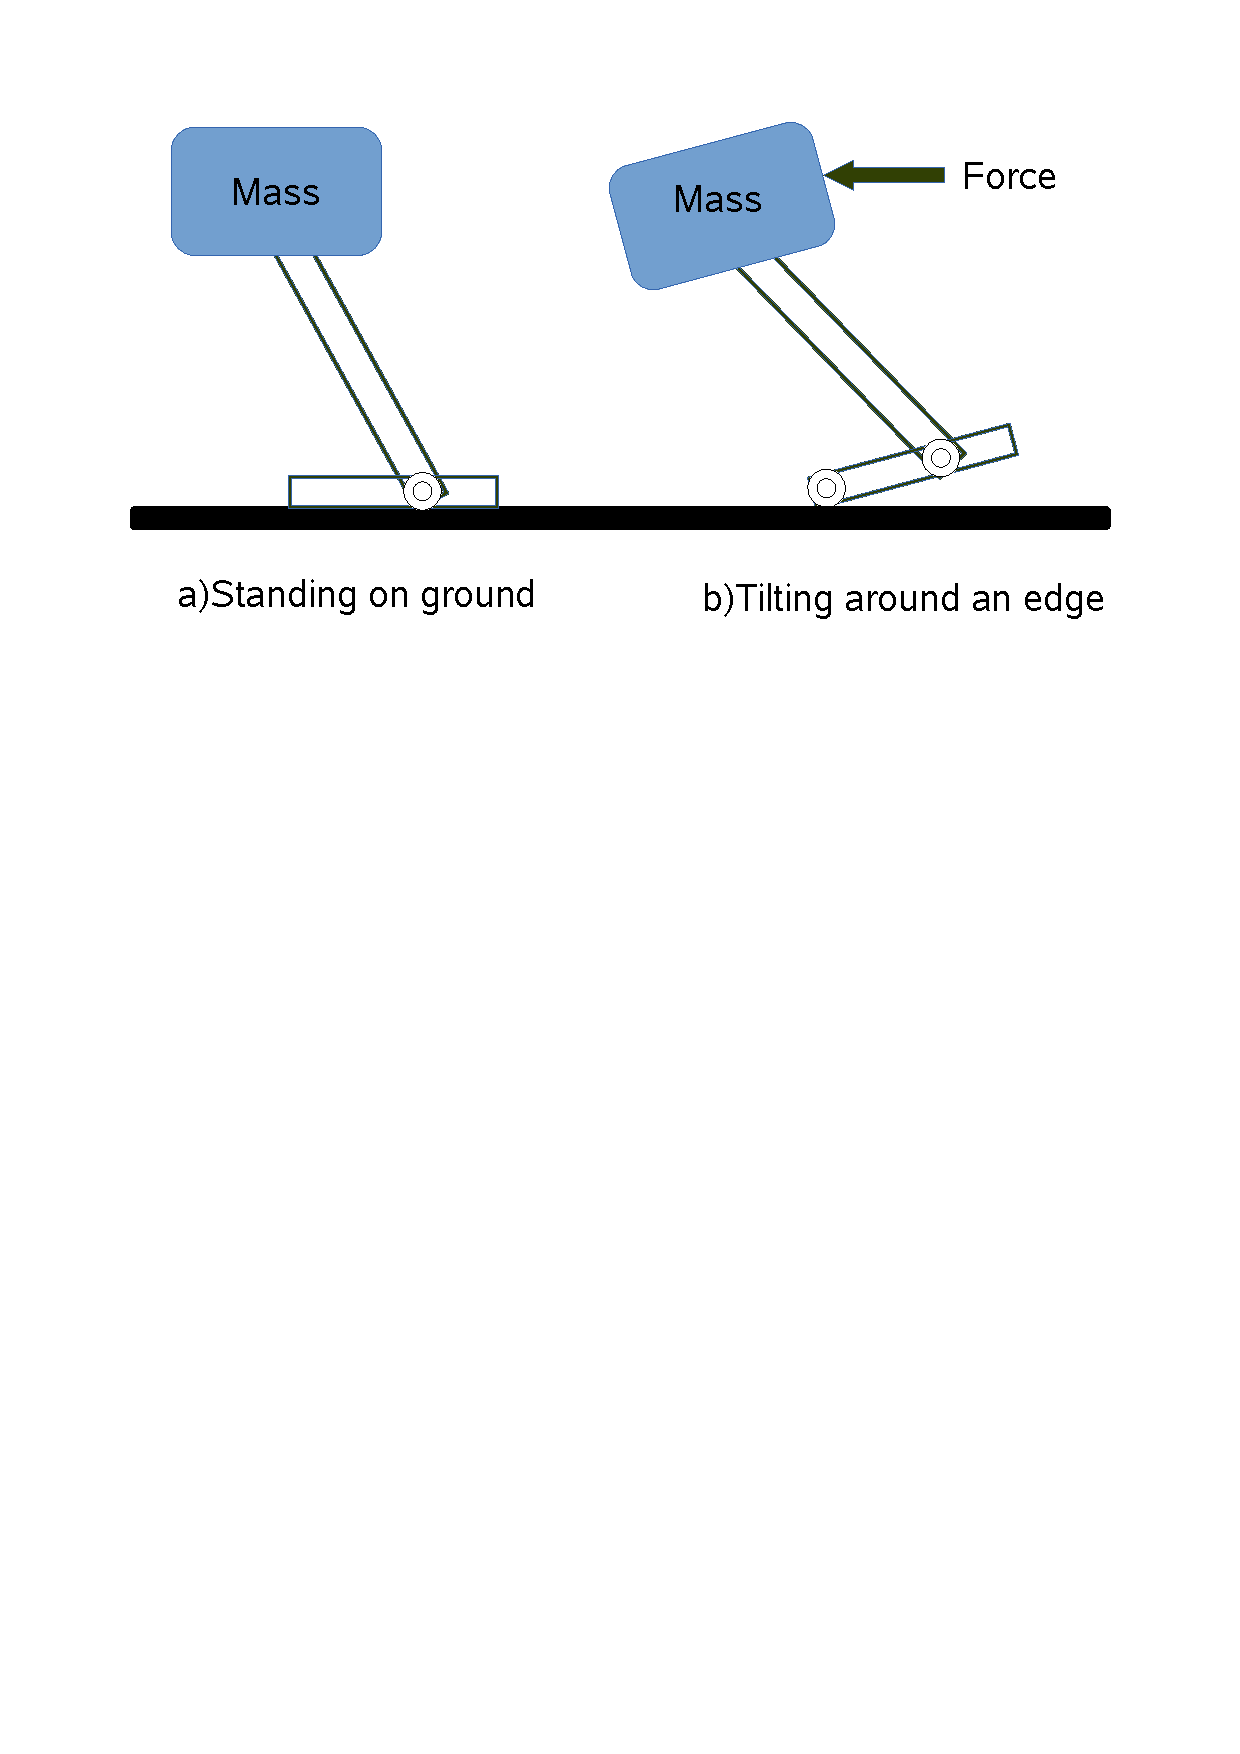
\includegraphics[trim = 0mm 180mm 0mm 10mm, scale=0.50]{Bilder/simp_uactcase.pdf}
	\caption{A simplified humanoid robot standing on one foot}
	\label{fig:idp_scene}
\end{figure}
Inorder to check the feasibility of solving the state estimation problem with the available measurements, a preliminary subproblem is formulated. Since we are interested in estimating the underactuated degrees of freedom, we have to consider the senario where these underactuated degrees of freedom are action on the robot. Let us consider the senario where the robot is tilting around an edge of the foot by applying some external force as shown in Figure \ref{fig:idp_scene}.b. All the joints other that ankle joint of the robot are assumed to remain static(joints does not produce any motion) throughout the experiment. The kinematics of the robot is simplified to one joint on the ankle connecting the whole body with the foot as shown in \ref{fig:idp_scene}.a. The kinematics of \emph{Toro} is shown in Figure \ref{fig:toro_kin}. The mass block in the Figure \ref{fig:idp_scene} represents the inertia of upperbody. The inertia of leg is incorporated in the link connceting upperbody and foot. 

When the robot is tilting around an edge of the foot as shown in Figure \ref{fig:idp_scene}.b, we assume there is an imaginary joint located at the edge of the foot around which the robot tilts. Figure \ref{fig:idp_scene}.b resmbles an inverted double pendulum in Figure \ref{fig:idp}.
\begin{figure}[H]
	\centering
	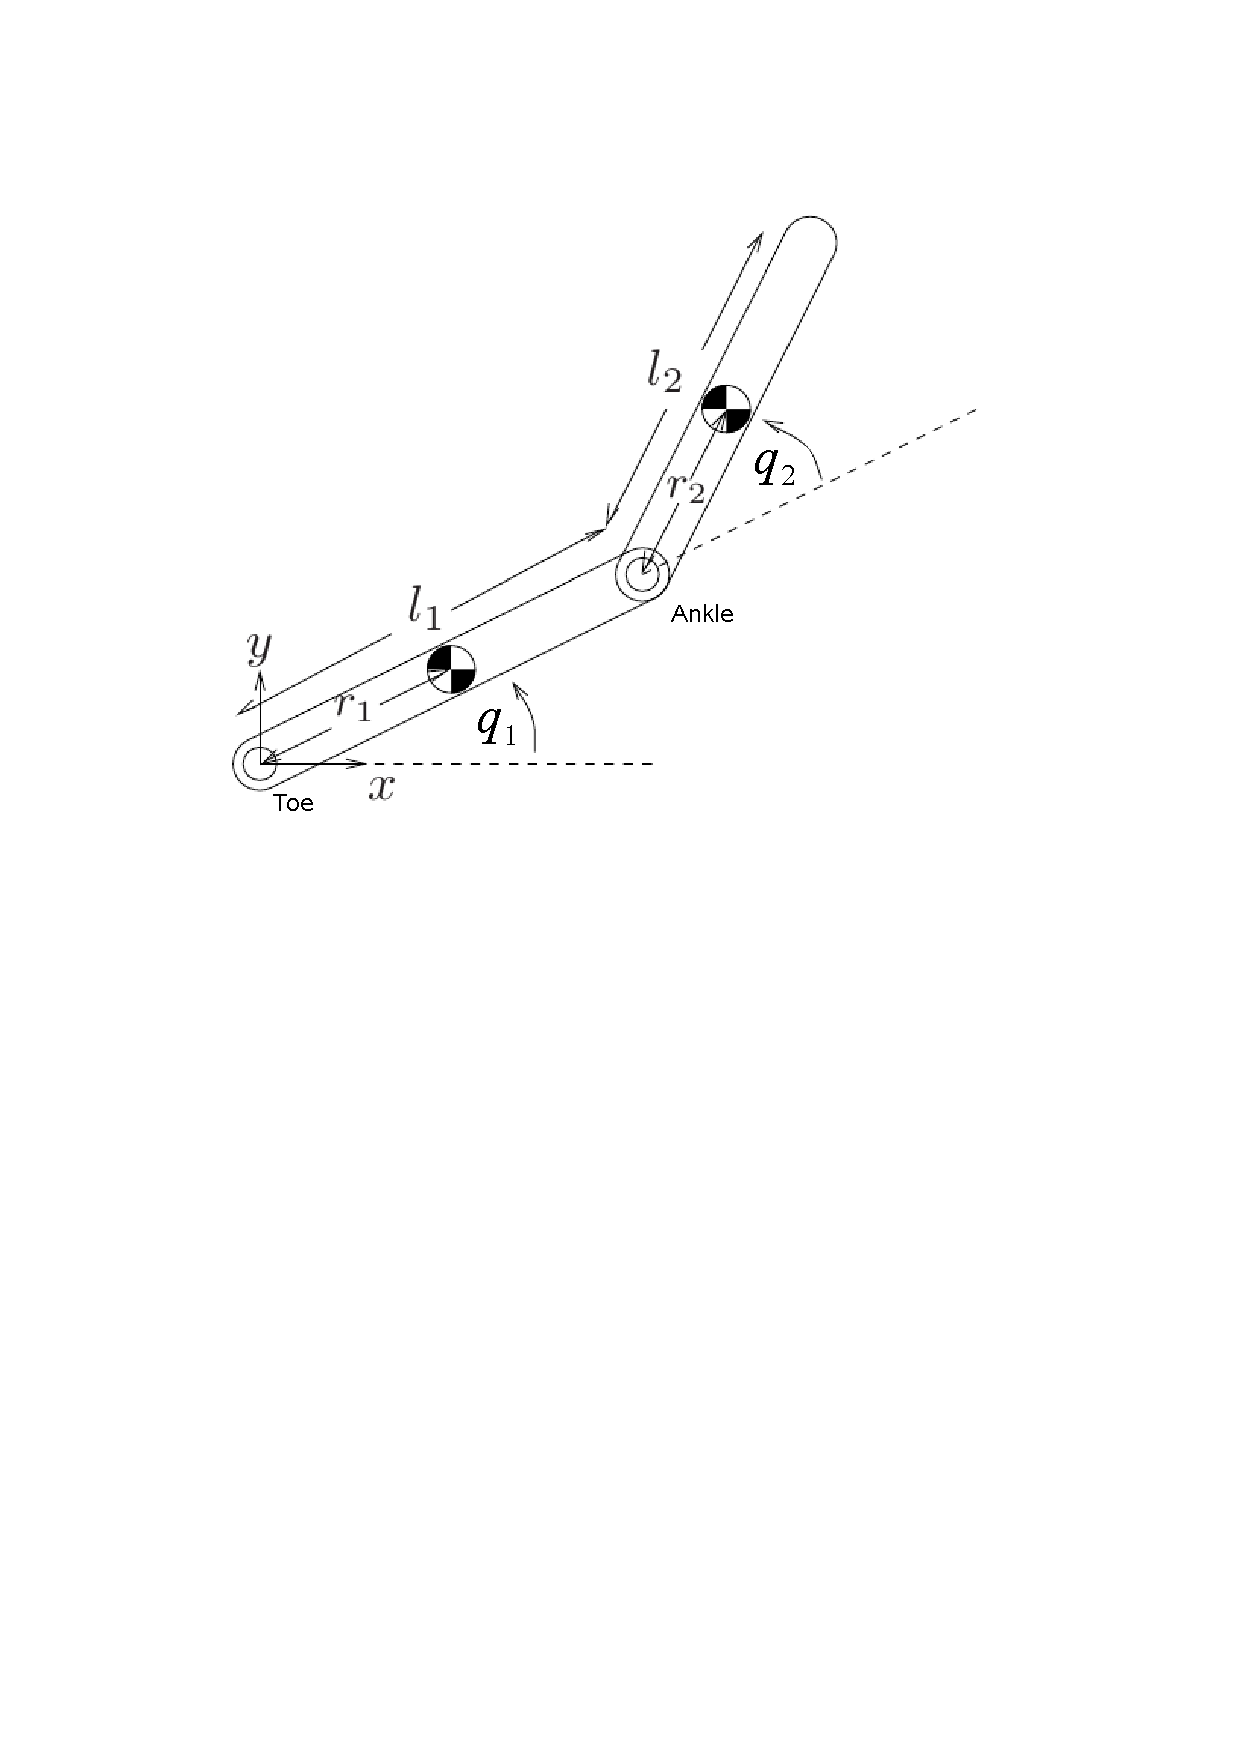
\includegraphics[trim= 0mm 150mm 0mm 0mm, scale=0.65]{Bilder/inv_db_pend.pdf}
	\caption[Inverted Double Pendulum]{Inverted Double Pendulum \footnotemark}
	\label{fig:idp}
\end{figure}
\footnotetext{Image source: A mathematical introduction to robotic manipulation \cite[Chapter 4, Page 164]{mur94}}
 The inverted double pendulum shown in Figure \ref{fig:idp} consists two links of length $l_1$ and $l_2$. The distance between center of mass of link 1 from the toe joint is $r_1$, $r_2$ is the distance between center of mass of link 2 from the ankle joint. In the inverted pendulum model the ankle joint is actuated but the toe joint is unactuated. The degrees of freedom of this model are toe and ankle. Toe is the underactuated degree of freedom whose motion parameters such as angle $q_1$ and angular velocity $\dot{q}_1$ needs to be estimated. The motion parameters of the inverted double pendulum are 
\begin{equation}
	 q = 
	\begin{pmatrix}
		q_{1}\\
		q_{2}
	\end{pmatrix}
	 \dot{q} = 
	\begin{pmatrix}
		\dot{q_{1}}\\
		\dot{q_{2}}
	\end{pmatrix},
\end{equation}
where \emph{q} is the vector of joint angles and $\dot{q}$ is the vector of joint angular velocities. The angle $q_1$ and angular velocity $\dot{q}_1$ are the motion parameters of toe joint. Likewise $q_2$ and $\dot{q}_2$ are the motion parameteres of ankle joint. The control input or torque applied to the ankle joint is $\tau$. 

The equation of motion of the inverted double pendulum is derived using Lagrange formulation given in Equation \ref{eq:lagrange}. The generalized coordinates of the system are $q_1$ and $q_2$, the velocities of the corresponding generalized coordinates are $\dot{q_1}$ and $\dot{q_2}$ as shown in Figure \ref{fig:idp}. The equation of motion of double pendulum written in general formulation of multi body system in Equation \ref{eq:dyn_mul_bdy} is, 
\begin{equation}
   \label{eq:dyn_idp}
	M(q_1,q_2)
	\begin{bmatrix}
		\ddot{q_{1}} \\
		\ddot{q_{2}} 
	\end{bmatrix}
	+ C(q_1,q_2,\dot{q}_1,\dot{q}_2)
    \begin{bmatrix}
		\dot{q_{1}} \\
		\dot{q_{2}} 
	\end{bmatrix}
	+ g(q_1,q_2) = 
    \begin{bmatrix} 0 \\ \tau \end{bmatrix},
\end{equation}
where, $M(q_1,q_2)$ represents the ineria matrix of the inverted double pendulum system. It is given by 
$$ M(q_1,q_2) = \begin{bmatrix}\
    \alpha+2\beta cos(q_2) & \delta + \beta cos(q_2) \\ 
    \delta + \beta cos(q_2) & \delta  \end{bmatrix},$$ where the terms $\alpha, \beta, \delta$ is given by
    $$
    \begin{aligned}
    \alpha &= \frac{1}{12} m_1 l_1^2 + \frac{1}{12} m_2 l_2^2 + m_1 r_1^2 + m_2 (r_2^2 + l_1^2),\\
    \beta &= m_2 l_1 r_2, \\
    \delta &= \frac{1}{12} m_2 l_2^2 + m_2 r_2^2.
    \end{aligned}
    $$
$C(q_1,q_2,\dot{q}_1,\dot{q}_2)$ represents the Corioli matrix of the system. It is given by 
$$C(q_1,q_2,\dot{q}_1,\dot{q}_2) = 
\begin{bmatrix}
-\beta sin(q_2) \dot{q}_2 &-\beta sin(q_2)(\dot{q}_1 + \dot{q}_2) \\
-\beta sin(q_2) \dot{q}_1 & 0
\end{bmatrix},
$$
where $\beta$ is given in the previous equation. The gravity vector is represented by $g(q_1,q_2)$. It is given by
$$g(q_1,q_2) = 
\begin{bmatrix}
(m_1 r_1 +m_2 l_1)a_g cos(q_1) + m_2 r_2 a_g cos(q_1+q_2) \\
m_2 l_2 a_g cos(q_1+q_2)
\end{bmatrix}
$$
where $a_g$ represents the acceleration due to gravity 9.81 $m/{s}^2$.

The state space representation of the inverted double pendulum system is formulated as given in Equation \ref{eq:dyn_ss}. The states of the system are $$ x = \begin{bmatrix} q_1 \\ q_2 \\ \dot q_1  \\ \dot q_2 \end{bmatrix}. $$

The measurement equation of the ODE system are formulated with the set of available measurements. The measurement equation is  
\begin{equation}
    \label{eq:y_idp}
	y= \begin{bmatrix} q_2 \\ \dot q_2 \\ acc_x \\ acc_y \\ \omega \end{bmatrix},
\end{equation}
where $q_2, \dot{q}_2$ are  angle and velocity of ankle joint measured by encoders. $acc_{x},acc_{y} $ are the Cartesian accelerations along \emph{x and y axis} measured by accelerometer present in inertial measurement unit(IMU) that is located at the end of link 2 in Figure \ref{fig:idp}. The acceleration measurements can be written in terms of states of the system as,
$$ 
    \begin{aligned}
    acc_x &= -l_1 (\ddot q_1 sin(q_1) + \dot q_1^2 cos(q_1)) - ((\ddot q_1 + \ddot q_2) l_2 sin(q_1+q_2) + (\dot q_1 + \dot q_2)^2 l_2 cos(q_1+q_2)), \\
    acc_y &= l_1 (\ddot q_1 cos(q_1) - \dot q_1^2 sin(q_1)) + ((\ddot q_1 + \ddot q_2) l_2 cos(q_1+q_2) - (\dot q_1 + \dot q_2)^2 l_2 sin(q_1+q_2)), \\
    \end{aligned}
$$
where $\ddot q_1 , \ddot q_2 $ are the accelerations which is computed using forward dynamics equation. The angular velocity of the whole system $\omega$ is measured by the gyroscope present in IMU. The measurement equation of the gyroscope is $$ \omega = \dot q_1 + \dot q_2. $$ 
The estimated states $$q_1, \dot{q_1}$$ are the angle and anglular velocity of the toe or the underactuated degrees of freedom of the system.

\subsection{Experiment}
\begin{figure}[h]
    \centering
    % We need layers to draw the block diagram
\pgfdeclarelayer{background}
\pgfdeclarelayer{foreground}
\pgfsetlayers{background,main,foreground}

% Define a few styles and constants
\tikzstyle{sensor}=[draw, fill=blue!20, text width=5em,text centered, minimum height=2.5em]
\tikzstyle{system} = [sensor, text width=6em, fill=green!30, 
    minimum height=12em, rounded corners]
\tikzstyle{input} = [coordinate]
\tikzstyle{sum} = [draw, fill=blue!20, circle, node distance=1cm]
%\tikzstyle{output} = [coordinate]
\def\blockdist{0.5}
\def\edgedist{0.75}
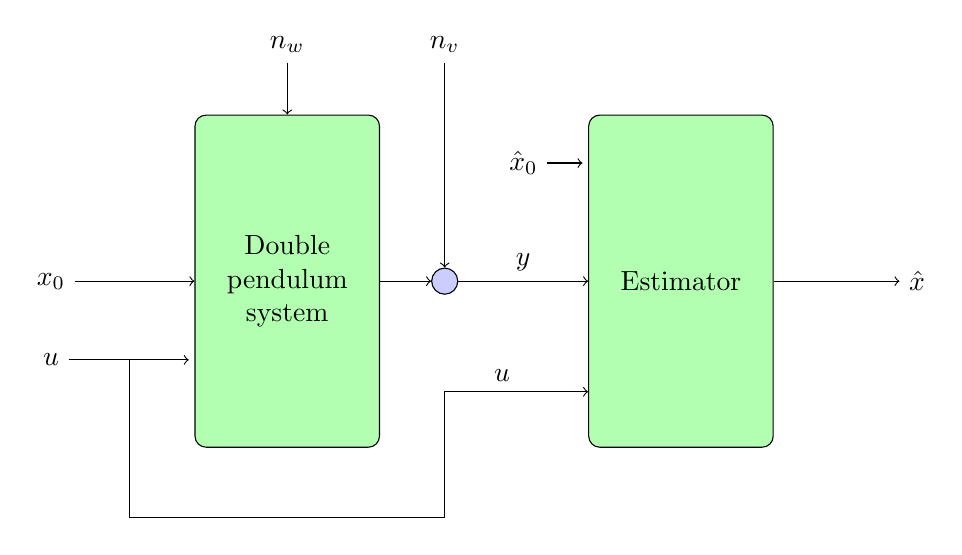
\begin{tikzpicture}
	% Define the nodes in the picture
	\node (sys_in)[yshift=1cm]{$x_0$};
	\node (u_in) [below of=sys_in,node distance=1cm]{$u$};
	\node (sys_u)[input,right of=u_in,node distance=1cm]{};
    \node (sim_sys) [system,right of=sys_in,node distance=3cm] {Double pendulum system};
    \node (sys_noise)[above of=sim_sys,node distance=3cm]{$n_w$};
    \node (msr_noise)[right of=sys_noise,node distance=2cm]{$n_v$};
    \node (msr_add)[sum,right of=sim_sys,node distance=2cm]{};
    \node (estimator) [system,right of=msr_add,node distance =3cm]{ Estimator};
    \node (est_in) [right of=sim_sys,node distance=3cm,yshift=1.5cm]{$\hat{x}_0$};
    \node (est_u) [input,right of =sim_sys, node distance=2cm,yshift=-3cm]{foo};
    \node (est_out)[right of=estimator,node distance=3cm]{$\hat{x}$};
    
    % Define the edges in the picture
    \draw [->] (sys_in) --node{}(sim_sys.west);
    \draw [-] (u_in) --node{}(sys_u);
    \draw [->] (sys_u) --node{}+(\edgedist,0);
    \draw [-] (sys_u) |-node{}(est_u);
    \draw [->] (est_u) |-node[pos=0.7,above]{$u$}(estimator.-130);
    \draw [->] (est_in) --node{}+(\edgedist,0);
    \draw [->] (sys_noise) --node{}(sim_sys.north);
    \draw [->] (msr_noise) --node{}(msr_add.north);
    \draw [->] (sim_sys.east) --node[above]{}(msr_add.west);
    \draw [->] (msr_add.east) --node[above]{$y$}(estimator.west);
    \draw [->] (estimator) --node{}(est_out);
\end{tikzpicture}
    \caption{Experimental setup of inverted double pendulum}
    \label{fig:exp_idp}  
\end{figure}

The state estimation problem is tested using Matlab Simulink. The experimental setup consists of the pendulum system and the state estimator. The pendulum system simulates the dynamical Equations \ref{eq:dyn_idp} of the inverted double pendulum system and outputs the measurements $y$ in Equation \ref{eq:y_idp}. Zero mean Gaussian white noises $n_w$ and $n_v$ are added to the state and measurements equations, so that the simulated system behaves closer to the real system. The state space equations of the pendulum system is 
\begin{equation}
    \label{eq:sim_idp}
    \begin{split}
    \dot x &= f(x,u) + n_w \\
    y &= h(x,u) + n_v.
    \end{split}
\end{equation}
Zero mean gaussian white noise of covairance $n_w$ and $n_v$ are added to the process and measurements of inverted double pendulum system.The table below lists the variance of the process and measurement noises used in the experiment.
\begin{table}[H]
    \centering
    \begin{tabular}{|c|c|}
    \hline
    Noise &Variance\\ \hline
    \textbf{Process noise $w_n$:}&\hspace{2mm} \\
    $\dot q_2$ &$1e^{-3}$ \\ \hline
    \textbf{Measurement noise $v_n$:}&\hspace{2mm} \\
     $acc$ &$1e^{-2}$ \\
     $gyro$ &$1e^{-4}$ \\
     $q$ &$1e^{-6}$\\ 
     $\dot q$ &$1e^{-6}$ \\ \hline
    \end{tabular}
    \caption{ Variance of the Gaussian white noise}
    \label{tab:idp_noise}
\end{table}

%\subsubsection{EKF}
 The equations of continuous time extended kalman filter is given in Equation \ref{eq:ekf_con}. The non linear state space equation of the system is given in Equations \ref{eq:dyn_ss} and \ref{eq:y_idp}. The Jacobians matrices $A$ and $H$ are computed with the help of symbolic toolbox in Matlab.

In Figure \ref{fig:exp_idp}, $x_0$ and $\hat x_0$ are the initial states of the system and estimator. The input $\tau$ applied is applied to the ankle joint. The system and estimator are initialzed with different initial values. 
$$ x_0 = \begin{bmatrix} 0.9575 \\ 0.9649\\ 0.1576\\ 0.9706 \end{bmatrix}, \hat x_0 = \begin{bmatrix} 0 \\ 0\\ 0\\ 0 \end{bmatrix}.$$  
The initial values of the error covariance matrix $P$ is $$P_0 = I_4, $$ where $I_4$ is a $4 \times 4$ identity matrix.


The process covariance $Q$ and measurement covariance $R$ matrices of the EKF are assigned with the corresponding values of measurement and process noise variance's in Table \ref{tab:idp_noise}.
$$  \begin{aligned}
    Q&=diag([0; 0; 0; 1e^{-3}]) \\
    R&=diag([1e^{-2}; 1e^{-4}; 1e^{-6}; 1e^{-6}]) \\
    \end{aligned}
    $$

The following tuning parameters are set for UKF:
$$  \begin{aligned}
    \alpha = 1 \\
    \beta = 0\\
    \kappa = -1 
    \end{aligned} $$ 
% Make a plot of the noise and actual measurement data here %
The whole system is simulated for 10 seconds with time step of 1 millisecond.
\subsubsection{Observation}
\begin{figure}
	\centering
	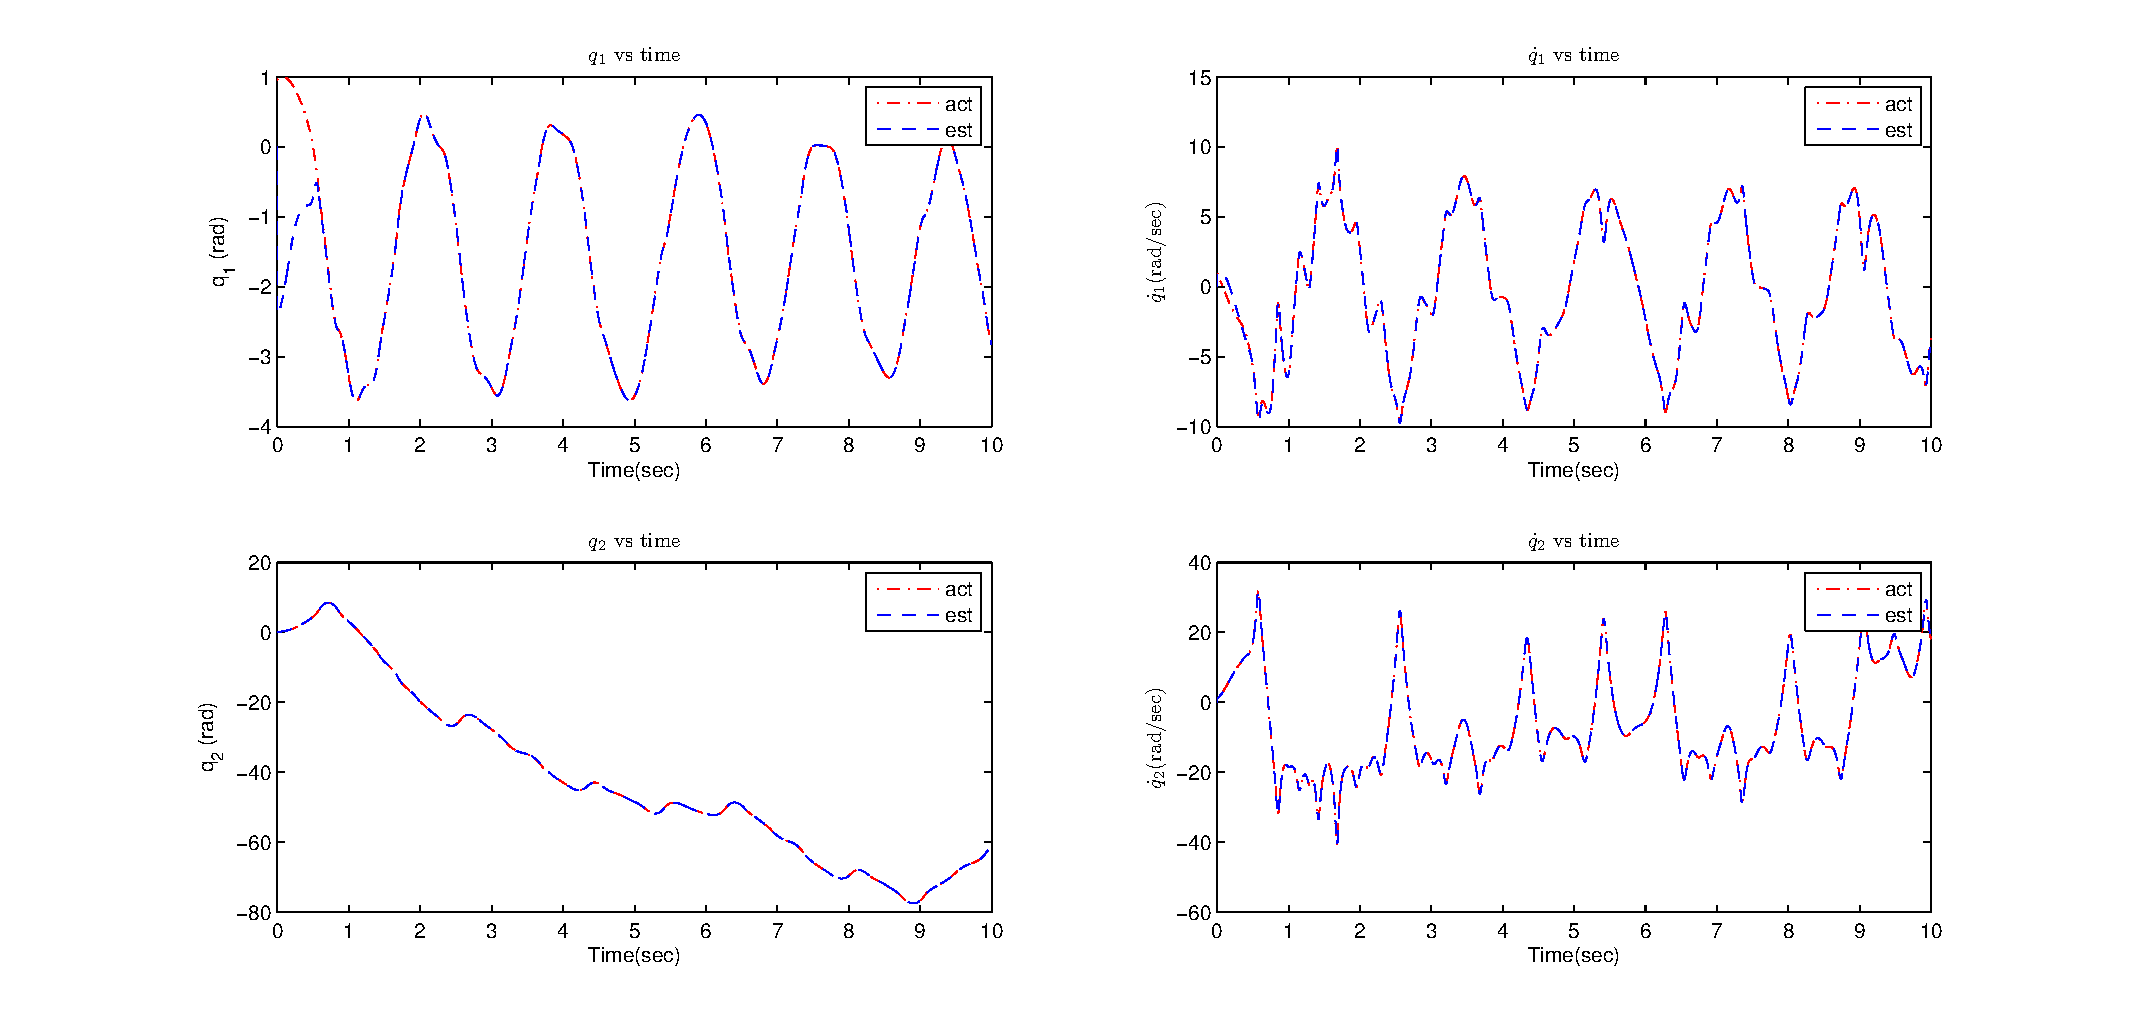
\includegraphics[angle=90,scale=0.5]{Bilder/plots/idp/idp_plot.pdf}
	\caption{ Plots of estimated state $\hat x$ and true state $x$ vs time}
	\label{fig:idp_plot}
\end{figure}

From the plots in Figure \ref{fig:idp_plot} it can be seen that the actual states and estimates converges to same value after some time. This implies the system is observable for the given measurements. 
\begin{figure}
    \centering
    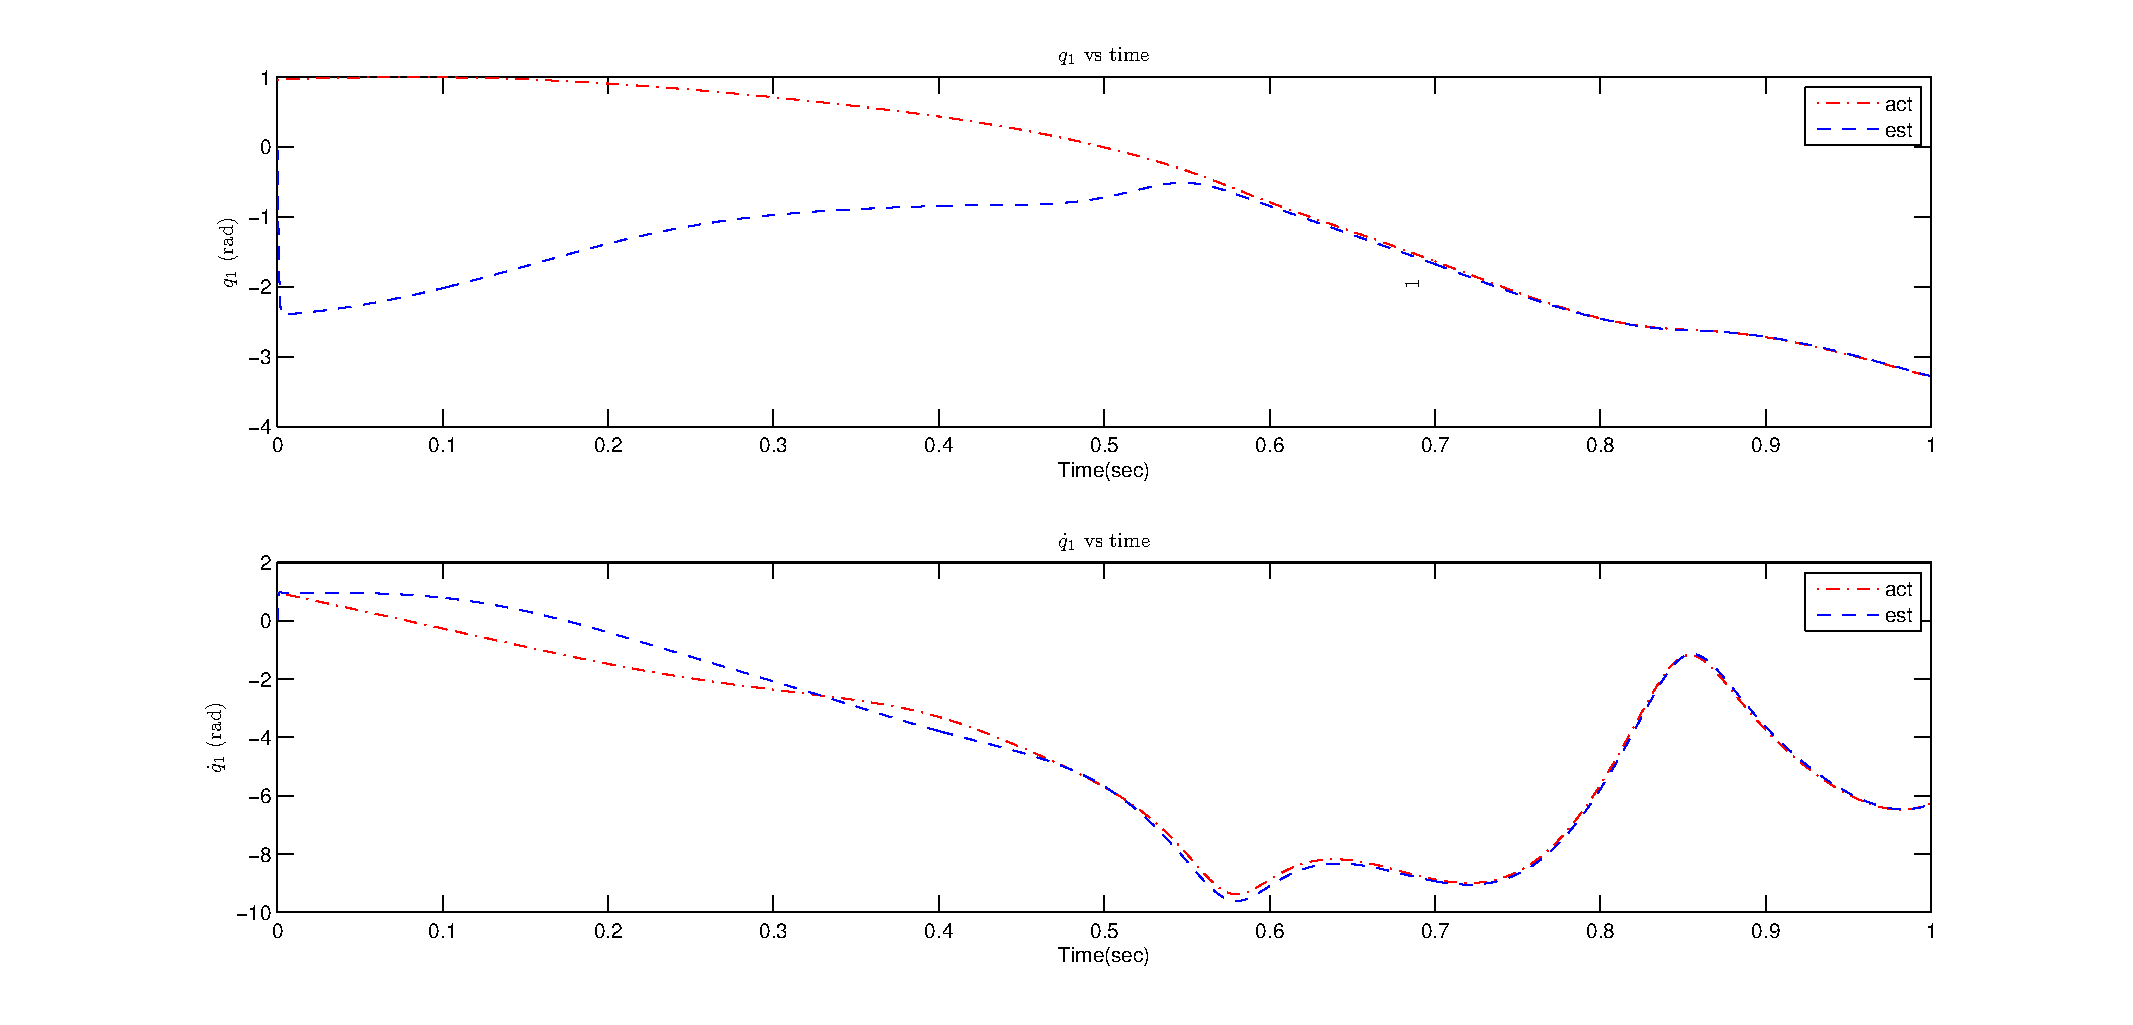
\includegraphics[trim= 30mm 0mm 30mm 0mm,clip,width=\linewidth]{Bilder/plots/idp/init_beh.pdf}
    \caption{ Convergence of the estimates to actual states }
    \label{fig:idp_init_conv}
\end{figure}
The initial convergence of the estimates is shown in Figure \ref{fig:idp_init_conv}. Filter converges in $0.6 sec$ for the given setting of $P_0=I_4$. When the initial error covairance is decreased to $\frac{1}{2}P_0$ the the time taken for convergance increases to $2 sec$. 

\begin{table}[H]
    \centering
    \begin{tabular}{|c|c|}
    \hline
    Estimates &RMSE \\ \hline
    $\hat q_1$   &0.0045 \\ \hline
    $\hat {\dot q}_1$ & 0.0261 \\ \hline
    \end{tabular}
    \caption{RMSE values for EKF estimates}
    \label{tab:idp_rmse_ekf}
\end{table}

\begin{table}[H]
    \centering
    \begin{tabular}{|c|c|}
    \hline
    Estimates &RMSE \\ \hline
    $\hat q_1$   &0.0045 \\ \hline
    $\hat {\dot q}_1$ & 0.0332 \\ \hline
    \end{tabular}
    \caption{RMSE values for UKF estimates}
    \label{tab:idp_rmse_ukf}
\end{table}

\begin{table}[H]
    \centering
    \begin{tabular}{|c|c|}
    \hline
    Estimator &Time(sec) \\ \hline
    $EKF$ &24 \\ \hline
    $UKF$ &30 \\ \hline
    \end{tabular}
    \caption{Time taken for 10 seconds simulation}
    \label{tab:idp_sim_time}
\end{table}
The root mean square error (RMSE) value of the states $\hat q_1, \hat{\dot q}_1 $ estimated by EKF and UKF are given in Tables \ref{tab:idp_rmse_ekf} and \ref{tab:idp_rmse_ukf}. Both the UKF and EKF has the same performance in esimating $\hat q_1$ but EKF performs better in estimating $\hat{\dot q}_1$. The time taken for simulation of the EKF is lesser than UKF. The simulation time of UKF depends upon the number of states. The number of sigma points requrired to approximate the nonlinear function is given by $2n+1$.
